\documentclass[11pt,a4paper]{article}
%\textheight = 630pt
%\textwidth = 480pt
%\topmargin = 3pt
%\voffset = 0pt
%\headsep = 2pt
%\headheight = 1pt
%\oddsidemargin = 1pt
%\marginparwidth = 1pt

%% Save space packages and settings %%
\usepackage{cite}

\usepackage{paralist}
\usepackage[compact]{titlesec}
\titlespacing{\section}{0pt}{0.5ex}{0.5ex}
\titlespacing{\subsection}{0pt}{0.5ex}{0ex}
\titlespacing{\subsubseSction}{0pt}{0.5ex}{0ex}
\linespread{0.9}

\usepackage{changepage}
\usepackage[hmargin=2cm, vmargin=2cm]{geometry}
\usepackage{parskip}
\setlength{\parskip}{5pt}
\usepackage{fancyvrb}
\usepackage{graphicx}
\usepackage{amsmath}
\usepackage{capt-of}
\usepackage{amsfonts}
\usepackage{verbatim}
\usepackage{courier}
\usepackage{float}
\restylefloat{table}

%%%%%%%%%%%%%%%%%%% Code %%%%%%%%%%%%%%%%%%%%%
\usepackage{color}
\usepackage[table]{xcolor} %adding background color to your tables
\usepackage{listings}% Allows you to present C++ syntax as it looks
\usepackage{listings} %enables inputing code set the settings below
\definecolor{dkgreen}{rgb}{0,0.45,0}
\definecolor{gray}{rgb}{0.2,0.5,0.5}
\definecolor{mauve}{rgb}{0.58,0,0.82}
%\definecolor{purple}{RGB}}{204, 45, 109}
\lstset{ %
language=C, % choose the language of the code
commentstyle=\color{dkgreen},
basicstyle=\footnotesize\ttfamily, % the size of the fonts that are used for the code
numbers=left, % where to put the line-numbers
numberstyle=\footnotesize, % the size of the fonts that are used for the line-numbers
stepnumber=1, % the step between two line-numbers. If it is 1 each line will be numbered
numbersep=5pt, % how far the line-numbers are from the code
backgroundcolor=\color{white}, % choose the background color. You must add \usepackage{color}
showspaces=false, % show spaces adding particular underscores
showstringspaces=false, % underline spaces within strings
showtabs=false, % show tabs within strings adding particular underscores
frame=single, % adds a frame around the code
tabsize=2, % sets default tabsize to 2 spaces
captionpos=b, % sets the caption-position to bottom
breaklines=true, % sets automatic line breaking
breakatwhitespace=false, % sets if automatic breaks should only happen at whitespace
keywordstyle=\color{purple}, % keyword style
numberstyle=\tiny\color{gray}, % the style that is used for the line-numbers
rulecolor=\color{black}, % if not set, the frame-color may be changed on
stringstyle=\color{blue}, % string literal style
escapeinside={\%*}{*)} % if you want to add a comment within your code
}
\DefineVerbatimEnvironment{code}{Verbatim}{fontsize=\small}
\DefineVerbatimEnvironment{example}{Verbatim}{fontsize=\small}
%%%%%%%%%%%%%%%%%%%%%%%%%%%%%%%%%%%%%%%%%%%%%%%%

\begin{document}

\title{Analysing London Twitter Data using Sparse PCA}
\author{
Theo Pavlakou\\ tp710\\ CID 00651782\\
}
\date{\today}
\maketitle
\pagenumbering{gobble}
\newpage

\section*{\center Abstract}

\clearpage
\pagenumbering{arabic}

\section{Introduction}
Social media now shapes our lives in such a vast way. More than $98\%$ of 18-24 year olds use social media, such as Facebook, Twitter and Instagram, and most use them more than half an hour a day on average\cite{statbrain}. Recently there has been a lot of work that has gone into analysing this vast amount of data that is available freely on the internet to understand trends in populations and to be able to target particular groups for marketing purposes. The term ``Big Data'' has become very widely used and the data that we encounter in these social media fit straight into this category. Machine learning algorithms and mathematical techniques can be used on this noisy data to find trends and infer useful results that can further be used to predict future trends. 
One such technique is known as Principal Component Analysis (PCA) and is concerned with finding which features in a vector lead to the highest variation, which in turn means leading to the highest information gain. The problem with PCA can be hard to interpret since the size of the vector that is returned could be immense in length (e.g. 3000 components) with only a few being of significance. This has led to the creation of algorithms that return sparse representations approximating the principal components, but which lead to results that are much easier to interpret. In this project the algorithms currently present to perform sparse PCA are analysed, evaluation of one such algorithm against a batch of Twitter data gathered from London in 2012 is then performed and then methods of improvement to the algorithm are also considered and methods to scale it. 

%% Mention only if reference is found
%Lots of money goes into this yearly, and companies such as Google and Facebook spend \textbf{(Find number and cite)} per year on such methods to maintain their competitive edge in industry. 

\section{Project Specification}

The purpose of this study is to examine how a certain implementation of Sparse PCA, described in \cite{dimakis}, can help to infer results from social media. The data used is a batch of Tweets from London throughout the year 2012. The reason Twitter data has been chosen is due to the word limit, which means that each Tweet is typically quite information dense, which is best to test the algorithm and come up with useful results in the first iteration. Later improvements may be used on lengthier texts, but a more sophisticated parser may need to be used in that scenario. After concluding meaningful results for the data as a whole, windowing the data into smaller periods of time is also attempted and an evolution of the results is examined further to see how the principal components correlate to events that happened in 2012. Measures to improve the algorithm's performance and the scalability of the algorithm are also explored.

\textbf{Not done:}
\begin{itemize}
\item What will be done next?
\end{itemize}


\section{Background}
To understand the project in detail, it is necessary to first understand some of the underlying methods that are used and the theory behind them. In this section, an attempt is made to give a thorough enough explanation whilst not going too in depth to diverge from the main topic of discussion. It also gives reasons as to why this project is important, what work has already been done in this field and why the particular direction has been chosen. 

\textbf{Not done:}
\begin{itemize}
\item Explain SVD in this scenario and how it relates (see http://people.cs.pitt.edu/~milos/courses/cs3750-Fall2007/lectures/PCA.pdf)?
\end{itemize}

\subsection{Related Work}
The idea of using social media as a medium for data analysis is not new and much work has been done in this area. Some particular examples are \cite{dimakis} and \cite{microblogs}. These two both lay a solid foundation for the work explored in this paper as it uses a lot of their findings and results and starts where they left off. For instance, the Sparse PCA algorithm is the same algorithm, with some slight modifications, as in \cite{dimakis} and the data used is the same data as was used in \cite{microblogs}. The focus of these however is quite different. In \cite{dimakis}, a lot more emphasis is put on the actual algorithm itself, whereas in this paper many other areas are explored, such as the trade-off between the number of features chosen, the number of points taken and the results obtained. Moreover, scalability is also considered in much more detail than in any of these. 

A lot of work has been done in the area of Sparse PCA as well. \cite{zou}, \cite{shen} and \cite{alex} (and many others) also come up with algorithms for Sparse PCA but, once again, focus a lot on the actual algorithm itself rather than the selection of the data that can be used for the algorithm. The reason the implementation in \cite{dimakis} has been used is due to the fact that it is faster for matrices with non-negative entries, by a factor of $2^{d-1}$, where $d$ is the number of principal components desired and also it has a feature elimination step which is used to make working on large data sets manageable. Furthermore, the data being used is Twitter data as the authors of \cite{dimakis} use also. 

\textbf{Not done:}
\begin{itemize}
\item Explain what has been done in more detail, including some of the maths.
\end{itemize}

\subsection{Principal Component Analysis (PCA)}
\subsubsection{Description}
Principal Component Analysis is a method that can be used to reduce the dimensionality of a data set by projecting it onto the principal subspace that is spanned by the eigenvectors with the largest eigenvalues of the covariance matrix. The reason that the largest eigenvalue eigenvectors are chosen is because these are the eigenvectors along which the largest variance occurs and therefore the most information can be retrieved from (see Appendix for a more thorough proof of this). This can be seen in Figure \ref{pca}. Here we have a two dimensional data set, say $\mathbf{S} \in \mathbb{R}^{m \times 2}$, where $m$ is the number of data points, which has been plotted on the first of the three graphs. It can be seen, however, that the points vary from the blue line only slightly, which means that, if the data can be projected onto this direction, the data can be approximated by only one component. When performing principal component analysis, the principal components that are found are:

\begin{equation*}
\mathbf{U} = 
\begin{pmatrix}
\mathbf{u}_1 && \mathbf{u}_2
\end{pmatrix} = 
\begin{pmatrix}
0.6956 && 0.7184\\
 0.7184 && -0.6956\\

\end{pmatrix}
\end{equation*}

We can then project the data onto the new principal components, as such:

\begin{equation*}
\mathbf{S}_p = \mathbf{S}\mathbf{U}
\end{equation*}
where $\mathbf{S}_p \in \mathbb{R}^{m \times 2}$ is the data projected onto the new principal components, namely $\mathbf{u}_1$ and $\mathbf{u}_2$. The plot of this new data can be seen in the second graph. 

In the third graph we project the data only onto $\mathbf{u}_1$ i.e.
\begin{equation*}
\mathbf{S}_p = \mathbf{S}\mathbf{u}_1
\end{equation*}

As it can be seen, this graph only differs by the second graph by a small amount but only half the features have been used. This is an example of dimensionality reduction (or compression). In this case, the number of features has been reduced to half the number before, but a lot more than half the variation has been maintained. In the application of PCA explored here, the second stage is more important, as the variation direction is what is considered most and not the compression, but this has been added for completeness. Another great explanation of PCA can be found in \cite{randomprojections}.

The first principal component (i.e. the first eigenvector of the $n\times n$ matrix, $\mathbf{A}$) is:
\begin{equation}
\mathbf{u}_1 = \underset{\|\mathbf{x}\|^2 = 1}{\operatorname{argmax}}\left( \mathbf{x}^T\mathbf{A}\mathbf{x}\right)
\end{equation}
Where $\mathbf{A} = \mathbf{S}^T\mathbf{S}$ and $\mathbf{S}$ is the $m\times n$ data set consisting of $m$ data points, each evaluated on $n$ features. An intuition to what $\mathbf{A}$ represents is presented in the Appendix. Principal Component Analysis alongside Singular Value Decomposition is explained further in \cite{datascience} and \cite{bishop}. 

\begin{figure}[H]
\centering
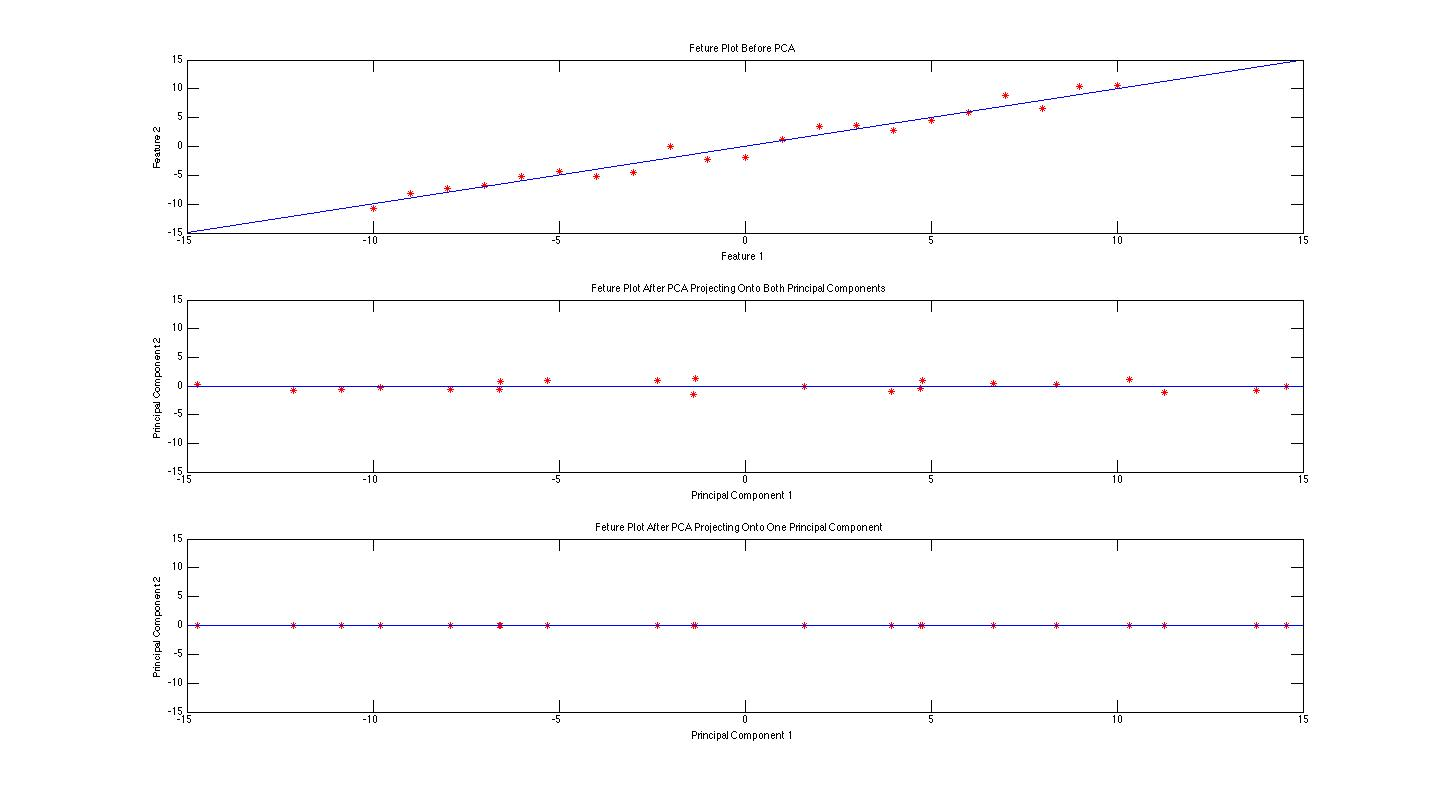
\includegraphics[scale=0.35]{PCA_EXPLAINED.jpg}
\caption{Images demonstrating what PCA is actually doing. The first image shows the plot of the features before performing the PCA. The second shows the features plotted on both the new principal components and the third shows the plot only plotted on the first principal compnent.}
\label{pca}
\end{figure}


\subsubsection{Sparse PCA}

Sparse PCA is a variant of PCA, which gives rise to principal components that only have few non-zero entries. The reason sparsity is desired in the eigenvectors is because sparse approximations of the eigenvectors are useful for interpreting data that have large dimensions. For example, in the specific application discussed in this paper, a set of words is considered and meaningful inferences are to be found from this data. It is clearly much simpler to analyse data given a small set of words that could approximate the variance in the given data set per principal component, than all the words in the data set which would contribute a small amount each, increasing the dimensionality of the principal component to the number of words in the set of all the words in all the Tweets. The equation to be solved resolves to:
\begin{equation}
\mathbf{u}_1 = \underset{\|\mathbf{x}\|_2^2 = 1, \|\mathbf{x}\|_0^2 = k}{\operatorname{argmax}}\left( \mathbf{x}^T\mathbf{A}\mathbf{x}\right)
\end{equation}
where $\|\mathbf{x}\|_0^2$ is the $l_0$ cardinality of $x$ i.e. how many non-zero elements x has. This is where Sparse PCA algorithms comes in. The one being used in this paper can be found in \cite{dimakis}.

\textbf{Not done:}
\begin{itemize}
\item Explain the algorithm used in \cite{dimakis}.
\item Explain one or two other algorithms also.
\end{itemize}

\subsection{Similarity to Singular Value Decomposition (SVD)}
This work is largely an extension of \ref{lecture_svd}.

\textbf{Should this be in the Appendix?}
\subsubsection{Description}
SVD is a decomposition method that is very important in many areas due to the way it breaks down a matrix into 3 matrices, each with a very informative structure. The basic concept is as such:
\begin{equation}
\mathbf{S} = \mathbf{U}\mathbf{\Sigma}\mathbf{V}^T
\end{equation}
Where $\mathbf{S} \in \mathbb{R}^{m \times n}$,  $\mathbf{U} \in \mathbb{R}^{m \times r}$ and is a column orthonormal matrix, where $r$ is equal to the rank of the matrix,  $\mathbf{V} \in \mathbb{R}^{n \times r}$ is also a column orthonormal matrix, and  $\mathbf{\Sigma} \in \mathbb{R}^{r \times r}$ is a diagonal matrix where the elements are sorted in descending order.

\subsubsection{Example Related to Project}
In the scenario considered in this paper, the matrix $\mathbf{S}$ is a matrix with the rows representing the tweets and the columns representing the words (features). The matrix is made up of only ones and zeros, with $\mathbf{S}_{i,j} = 1$, if tweet $i$ contains word $j$ and zero otherwise. As a toy example, suppose we have the matrix:
\begin{equation}
\mathbf{S} = 
\begin{pmatrix}
1 & 1 & 1 & 0 & 0\\
1 & 1 & 1 & 0 & 0\\
1 & 1 & 1 & 0 & 0\\
0 & 0 & 0 & 1 & 1\\
0 & 0 & 0 & 1 & 1\\
0 & 0 & 0 & 1 & 1\\
0 & 0 & 0 & 1 & 1\\
\end{pmatrix}
\end{equation}
Where the columns represent the ordered bag of words, referenced from left to right \{football, cup, win, cyprus, eu\}, and there are two main topics trending on Twitter. One is about some football victory, and the other is about Cyprus joining the EU. This is a very artificial example as it assumes that the tweets would contain the exact same words, but a more general example will be given later. As it can be seen, this matrix is of rank 2, which is also the number of topics that are presented by the matrix. 

Performing the SVD on the matrix, what is acquired is:

\begin{equation*}
\mathbf{S} = \mathbf{U}\mathbf{\Sigma}\mathbf{V}^T
\end{equation*}

\begin{equation}
\mathbf{S} = \begin{pmatrix}
-0.5774 & 0.0000\\
-0.5774 & 0.0000\\
-0.5774 & 0.0000\\
0.0000 & -0.5000\\
0.0000 & -0.5000\\
0.0000 & -0.5000\\
0.0000 & -0.5000\\
\end{pmatrix}
\begin{pmatrix}
3.0000 & 0.0000\\
0.0000 & 2.8284\\
\end{pmatrix}
\begin{pmatrix}
-0.5774 & -0.5774 & -0.5774 & 0.0000 & 0.0000 \\
0.0000 & 0.0000 & 0.0000 & -0.7071 & -0.7071\\
\end{pmatrix}
\end{equation}

These three matrices all have a very significant meaning. It has already been stated that due to the obvious form of $\mathbf{S}$ it can be seen that there are only 2 topics or concepts. The $\mathbf{U}$ matrix can be viewed as the Tweet to concept correlation matrix i.e. how correlated the Tweets are to the corresponding topics. Similarly, the $\mathbf{V}^T$ matrix can be viewed  the concept to word correlation matrix i.e. how related the concept is to the particular word. For example, $\mathbf{U}_{2,1}$ would be how related the second Tweet is to the first concept and $\mathbf{T}_{2,3}$ would be how related the second topic is related to the third word, which in this case is zero, i.e. there is no similarity, because the second concept is about Cyprus joining the EU and the third word is win, which does not appear in any Tweet regarding Cyprus and the EU. The $\mathbf{\Sigma}$ matrix is then just the concept strengths.

It can then be shown that $\mathbf{S}^T\mathbf{S}$ represents the correlation of the words in the tweets to each other, i.e. a covariance matrix (see Appendix). But 
\begin{equation*}
\mathbf{S}^T\mathbf{S} = \mathbf{V}\mathbf{\Sigma}\mathbf{U}^T  \mathbf{U}\mathbf{\Sigma}\mathbf{V}^T
\end{equation*}
\begin{equation}
\mathbf{S}^T\mathbf{S} = \mathbf{V}\mathbf{\Sigma}^2\mathbf{V}^T
\end{equation}
which can be rewritten as:
\begin{equation}
\mathbf{S}^T\mathbf{S} = \mathbf{V}\mathbf{\Lambda}\mathbf{V}^T
\end{equation}
which essentially means that the columns of $\mathbf{V}$ are the eigenvectors of the matrix $\mathbf{S}^T\mathbf{S}$ and the diagonal values of $\mathbf{\Lambda}$ are the corresponding eigenvalues, which are the squares of the singular values found in $\mathbf{\Sigma}$.

As it can be seen, there is a close relationship between SVD and PCA, which uses the eigenvectors of the covariance matrix. Therefore, to find the principal components of a matrix $\mathbf{S}$, the SVD can instead be found and the principal components would be the columns of $\mathbf{V}$ (or of $\mathbf{U}$ if we want to find the principal components of $\mathbf{S}\mathbf{S}^T$) and the variances are given by squaring the singular values.

\subsubsection{Further Example Related to Project}
Suppose the matrix $\mathbf{S}$ instead looked like this:

\begin{equation}
\mathbf{S} = 
\begin{pmatrix}
1 & 1 & 1 & 0 & 0\\
1 & 1 & 1 & 0 & 0\\
1 & 1 & 1 & 0 & 0\\
0 & 0 & 0 & 1 & 1\\
0 & 0 & 0 & 1 & 1\\
0 & 0 & 0 & 1 & 1\\
0 & 0 & 0 & 1 & 1\\
1 & 0 & 0 & 1 & 0\\
1 & 1 & 1 & 0 & 0\\
0 & 0 & 0 & 1 & 1\\
0 & 0 & 0 & 1 & 1\\
0 & 0 & 0 & 1 & 1\\
1 & 0 & 0 & 1 & 1\\
\end{pmatrix}
\end{equation}
with the same words representing the columns as in the previous example. It can be seen here that there are now 4 linearly independent columns and therefore this matrix is of rank 4. 

The SVD then turns out to give:


\begin{equation*}
\mathbf{U}=
\begin{pmatrix}
-0.1216&0.4704&-0.1158&0.0223\\
-0.1216&0.4704&-0.1158&0.0223\\
-0.1216&0.4704&-0.1158&0.0223\\
-0.3241&-0.1199&-0.1320&0.0778\\
-0.3241&-0.1199&-0.1320&0.0778\\
-0.3241&-0.1199&-0.1320&0.0778\\
-0.3241&-0.1199&-0.1320&0.0778\\
-0.2336&0.1097&0.7963&0.5471\\
-0.1216&0.4704&-0.1158&0.0223\\
-0.3241&-0.1199&-0.1320&0.0778\\
-0.3241&-0.1199&-0.1320&0.0778\\
-0.3241&-0.1199&-0.1320&0.0778\\
-0.3888&0.0453&0.4363&-0.8102\\
\end{pmatrix}
\end{equation*}
\begin{equation*}
\mathbf{\Sigma}=
\begin{pmatrix}
4.1377&0.0000&0.0000&0.0000\\
0.0000&3.5113&0.0000&0.0000\\
0.0000&0.0000&1.1637&0.0000\\
0.0000&0.0000&0.0000&0.4426\\
\end{pmatrix}
\end{equation*}
\begin{equation*}
\mathbf{V}=
\begin{pmatrix}
-0.2679&0.5801&0.6613&-0.3930\\
-0.1175&0.5359&-0.3980&0.2014\\
-0.1175&0.5359&-0.3980&0.2014\\
-0.6987&-0.1949&0.2654&0.6352\\
-0.6422&-0.2261&-0.4189&-0.6008\\
\end{pmatrix}
\end{equation*}
As it can be seen here, it is significantly more difficult to actually be able to distinguish which words contribute significantly to each principal component due to the added noise that rows 8 and 13 give rise to. This, once again, highlights how important sparse principal components are since here the data is only $\in \mathbb{R}^{13 \times 5}$ and it is difficult to interpret, whereas in a real life scenario this is much larger in magnitude, and in the scenario considered in this paper this grows to be in the tens of thousands Tweets and thousands of words.

What is very useful to see, however, is that the singular values do decrease quite rapidly after the second one. These represent the square roots of the eigenvalues of the covariance matrix, so by squaring them the graph in Figure \ref{spectrum} is obtained.

\begin{figure}[H]
\centering
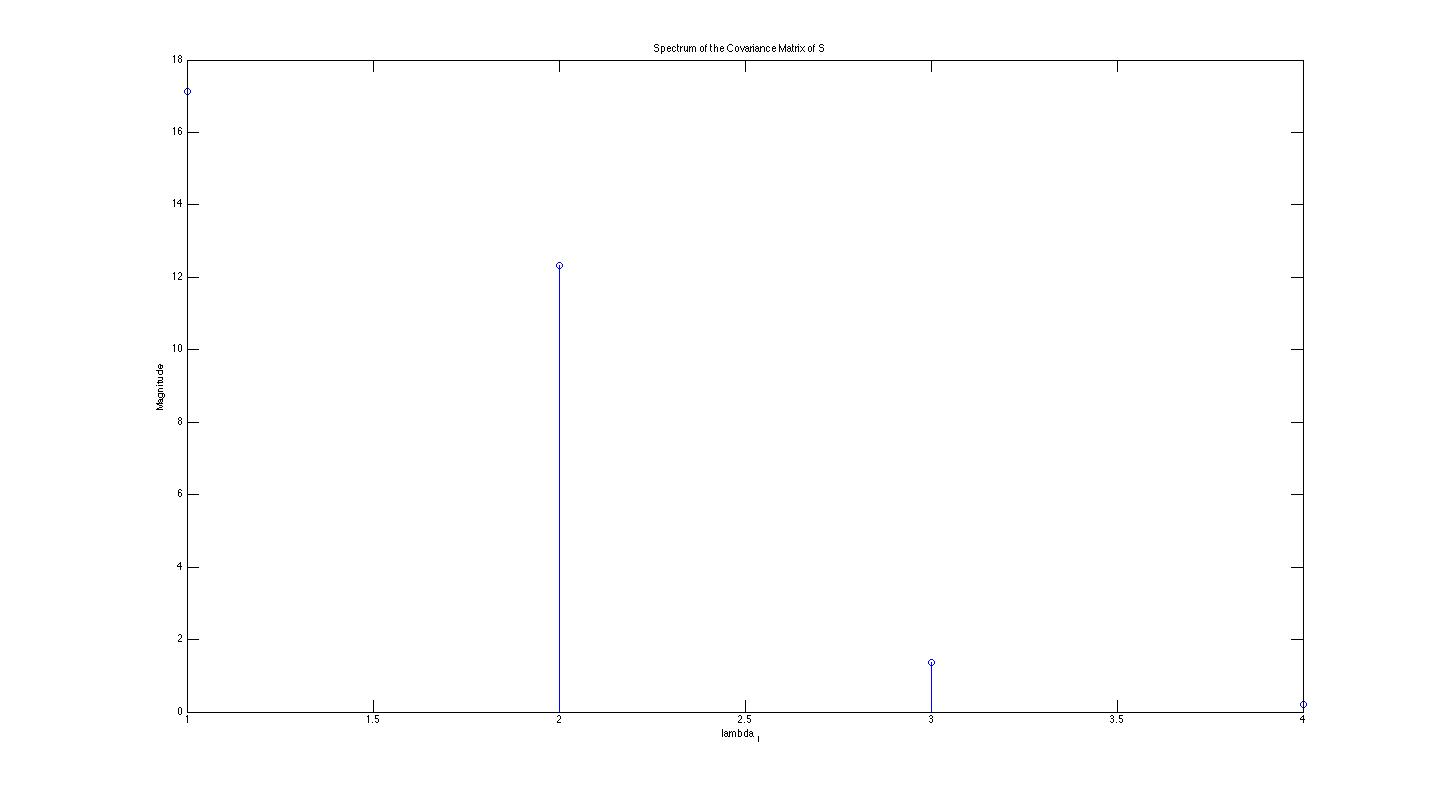
\includegraphics[scale=0.3]{Spectrum_Eigenvalues.jpg}
\caption{The spectrum of the eigenvalues of $\mathbf{S}^T\mathbf{S}$}
\label{spectrum}
\end{figure}

This intuitively makes sense since it is not hard to tell, after looking at the eigenvectors, that the first eigenvector is associated with the words Cyprus and EU, as 7 of the rows only mention these two words from the bag of words. The second eigenvector is associated with the words football, cup and win, as 4 of the rows only contain these words. These are obviously going to be the major concepts and so their eigenvalues are relatively quite high, with the first one being slightly higher. After these however, the eigenvalues fall significantly which relate to the added noise which is present due to the rows 8 and 13, since not much variance can be explained by these two eigenvectors and therefore they carry very little information. 
\clearpage
\section{Work Completed and Implementation Plan}

\subsection{The Bag-of-Words}
The choice of words to be chosen as the features must be carefully considered. For instance, one could simply take a union of all the words in the English dictionary, the words that are used on the internet, such as ``lol'' and ``yey'', and all the possible names of people and places, which would solve the problem of possibly missing out any features. This however would result in a matrix of immense dimension and therefore would be impossible to process, at least given any consumer computer. Therefore, some careful selection for the features must be exhibited so as to gain the features that carry the most information whilst still keeping the number of features to a manageable size. Some general guidelines for all methods are that words that typically do not give any additional information e.g. ``is'', ``the'', ``this'', etc. are to be eliminated. Furthermore, the Bag-of-Words should be completely independent of capital letters i.e. ``Road'' and ``road'' are to be considered equal. 

\subsubsection{Using Set of All Words in Tweets}
This first method attempts to use all the words that appear in the Tweets with the filter described above applied. Unfortunately, this results a set of over 78,000 features, which is much to large to process, so this method is not to be used. 

\subsubsection{Using Set of Three Thousand Most Common Words in the English Language}
The next method is to use a set of the 3,000 most common words in the English language as a whole. A problem with this is that, this list typically includes a lot of the very uninformative words, examples of which are given above, and does not include words that are not very common as a whole but, when some sort of event occurs, become very common, especially on social media. Furthermore, it also does not include any names or slang that is used on the internet. To illustrate, if Muse were to have a concert some time in June, it would be expected that a lot of Tweets may have the word ``Muse'' in them and ``concert'' and words like ``wow'' or ``amazing'', all of which are not in the top 3,000 words in the english language. Therefore, these features would be completly missed out and therefore a very valid principal component would possibly be non-existent in the final results.

\subsubsection{Adding Words in Tweets to the Bag-of-Words with a Certain Probability}
Another approach is to say that a word is added to the Bag-of-Words with a probability $p$. The intuition behind this is that words that do appear very often most probably will end up in the set, if p is large enough, but of the words that do not appear very often there would be less, giving a much more relevant bag of words and a much smaller set also (approximately $p$ times the size of the original).

We assume that all words are independent. Let $T_w$ be the event that we take the word $w$ and $A_{w, i}$ be the event that the word $w$ appears $i$ times and assume the probability of taking a word $w$, given that $w$ appears is $p$. 
\begin{equation*}
P\left( T_w | A_{w, i}\right) =  \sum_{j=1}^i {i \choose j} p^j\left( 1 - p\right)^{i-j}
\end{equation*}
which is equivalent to 
\begin{equation}
1 - P(T_w |  A_{w, i}) = 1 - (1 - p)^i
\end{equation}
%% Till here it has been checked and it is correct.
%and assume the probability of $w$ appearing is $q$, therefore the probability of $w$ appearing $i$ times is:
%\begin{equation}
%P\left(A_{w, i}\right) = q^i
%\end{equation}
%then the probability of taking the word $w$ is:
%\begin{equation*}
%P(T_w) = \sum_{i=1}^\infty P\left(T_w| \mathbf{A_{w, i}} \right) P( \mathbf{A_{w, i}})
%\end{equation*}
%\begin{equation}
%\sum_{i=0}^\infty P\left(T_w| \mathbf{A_{w, i}} \right) P( \mathbf{A_{w, i}}) =\sum_{i=1}^\infty \left(1 - (1 - p)^i\right) q^i
%\end{equation}

We can therefore see that the higher the occurrence of the word $w$, the higher the probability of it being added to the Bag-of-Words. Since popular events will have words associated with them that appear quite often, it can be said that with the right choice of $p$ (approximately 0.1), more informative words will appear in the Bag-of-Words, whilst also reducing the size of the set. 

This gives a final algorithm that is $O(N)$, where $N$ resembles the number of all the unique words in all the Tweets. 

This method seems to work to some extent, however, if the set of all the words grows too large, the probability $p$ will have to become much smaller to maintain a constant size for the Bag-of-Words. In turn, this means that the relevant words would have to occur more for them to be in the final set. This may not be the case however if taken over longer periods of time in which words associated with events may have large spikes for a few hours or days but when taken over the whole period of time, actually contribute a small percentage of the whole set of words.

\subsubsection{Taking $M$ Words of Highest Occurrence}

In this case, a set of words is created as before, but the frequency of each word in the set is also counted and the words are sorted in descending order of occurrence. When this is done, the first $M$ words are taken as the Bag-of-Words. The assumption here is that words that appear very often will be in the principal components, which is not completely justified, but empirically has been the case. For example, having taken the top 3000 words, the principal components always have words in the top 1000 words, most of which are in the top 500. This makes the computation feasible whilst still not losing a significant amount of information.

This is a $O(NlogN)$ algorithm, where $N$ resembles the number of all the unique words in all the Tweets. 

This suffers from the same problem as the probabilistic method, however, it ensures that words that do occur very frequently will be in the Bag-of-Words, as opposed to relying on probability. This method will be used from now on in this paper.

\subsection{The Matrix $\mathbf{A}$}

The matrix to be passed to the algorithm is also of interest, as it determines what sort of relationship the words have to one another. In this section, different versions of the matrix are considered and evaluated against each other so as to be used from here on. 

All testing is done using a subset of the Tweets, namely the first 1000 Tweets. This is roughly a day's worth of data. The algorithm is run on each of the matrices using the same parameters and 3 sparse PCAs are computed, each with 5 elements.
\subsubsection{The Initial Matrix $\mathbf{A}$}
The matrix which the sparse principal components are extracted from may take many forms. Initially, the approach considered in \cite{dimakis} is taken, in which $\mathbf{A} = \mathbf{S}^T \mathbf{S}$ where $\mathbf{S} \in \mathbb{R}^{m \times n}$ is the data matrix with $m$ rows as the Tweets and $n$ columns representing each of the words in the Bag-of-Words. However, different methods may also be explored which change the weightings of the features. 

\subsubsection*{Results}
\begin{table}[H]
\center
\begin{tabular}{| c l | c l | c l |}
\hline
Index & Word & Index & Word & Index & Word\\
\hline
2 & love & 3 & london & 1 & like\\
6 & know & 83 & hall & 9 & back\\
4 & people & 77 & royal & 44 & feel\\
1 & like & 9 & back & 13 & going\\
7 & don't & 166 & albert & 15 & follow\\
\hline
Eigenvalue & 44.4 & Eigenvalue & 35.1 & Eigenvalue & 33.1\\
\hline
\end{tabular}
\caption{The first 3 principal components using the algorithm on the initial matrix, $ \mathbf{A}$. The index represents the rank of the word according to how frequent the word is found in the all the tweets. The associated eigenvalue is also shown for each of the principal components.}
\end{table}

As it can be seen, two of the three principal components in this case do not really convey much information as to any particular event that took place and are just words that may be used together quite often but not especially when a certain event takes place, however the middle one does seem to give some insight. It seems to indicate that during the time these Tweets were created there was an event at the Royal Albert Hall in London. 

The eigenvalues also give some good insight and are useful for scoring the importance of different principal components. The higher the eigenvalue, the higher the variance this principal component accounts for, and therefore the more information it holds. In this scenario, the second principal component seems to get the second highest eigenvalue, which should be noted for the next case. 
  
\subsubsection{The Hollow Matrix $\mathbf{A}_{h}$}
As described in Appendix A, the matrix $\mathbf{A} = \mathbf{S}^T \mathbf{S}$ can be viewed as an undirected graph with each node being a word and each link being the number of times that word appears with the connecting word node in the same Tweet for all Tweets. This representation is meaningful, however the problem lies in the fact that the diagonal represents the number of times each word appears in total, regardless of any relation to the other words i.e. each node has a link to itself, with the highest weighting. This means that words that occur very frequently have very large values on their diagonal, regardless of how they relate to other words, which can be deceiving when taking the eigenvalues of the matrix. In attempt to prevent this, the matrix $\mathbf{A}$ can be substituted for 
$\mathbf{A}_h$ where for each of its elements, $a'_{i, j}$, it takes the value 

\begin{equation}
a'_{i, j} = 
\begin{cases}
a_{i, j} & \text{if}\ i \neq j\\
0 & \text{if}\ i = j
\end{cases}
\end{equation}
where $a_{i, j}$ are the elements in $\mathbf{A}$.

\subsubsection*{Results}
\begin{table}[H]
\center
\begin{tabular}{| c l | c l | c l |}
\hline
Index & Word & Index & Word & Index & Word\\
\hline
6 & know & 13 & going & 3 & london\\
7 & don't & 22 & some & 83 & hall\\
1 & like & 14 & sleep & 77 & royal\\
16 & about & 52 & **** & 166 & albert\\
4 & people & 102 & house & 124 & greater\\
\hline
Eigenvalue & 13.5 & Eigenvalue & 9.6 & Eigenvalue & 16.6\\
\hline
\end{tabular}
\caption{The first 3 principal components using the algorithm on the hollow matrix, $ \mathbf{A}_h$. The index represents the rank of the word according to how frequent the word is found in the all the tweets. The associated eigenvalue is also shown for each of the principal components.}
\end{table}

In this case, once again two of the three principal components are not very insightful but the third is again talking about the Royal Albert Hall in London. The interesting thing to not here is that the associated eigenvalue for the third principal component and the most useful is actually the highest. This, as suspected, means that this method gives significantly better results that the previous method.

\subsubsection{The Normalised Matrix $\mathbf{A}_{n}$}
Here, making the matrix have normalised rows is considered and the resulting matrix is $\mathbf{A}_n$. The basic concept is to make it so that all the rows/columns sum to 1 so that it does not matter which words actually appear the most, but how often they appear with other words relative to their weighting.

\subsubsection*{Results}

\begin{table}[H]
\center
\begin{tabular}{| c l | c l | c l |}
\hline
Index & Word & Index & Word & Index & Word\\
\hline
1782 & glisse & 2084 & cried & 1615 & iwalnut\\
1484 & mafia & 1692 & hollyoakslater & 2339 & arre\\
773 & volton & 873 & tonight's &2422 & abrazo\\
1008 & sons & 2382 & alkolik & 1351 & olmaden\\
2086 & conette & 900 & throuhout & 1711 & hermano\\
\hline
\end{tabular}
\caption{The first 3 principal components using the algorithm on the hollow matrix, $ \mathbf{A}_n$. The index represents the rank of the word according to how frequent the word is found in the all the tweets. }
\end{table}

Clearly this gives results that are absolutely irrelevant. The reason for this is because, now that all the words have been normalised, those that appear only a few times together with other words will get a higher weighting. For instance, if a word only appears once with another word, then it will get a value of 1 and, therefore will appear to give a higher variance than it does in actual fact. This method will not be considered from here on.

\subsection{Scaling the Method}
Until this point, the matrix $\mathbf{S} \in \mathbb{R}^{m \times n}$, where $m$ is the number of tweets and $n$ is the number of words in the bag of words, has to be very limited in size. This may work for the area of London as 40k Tweets corresponds to roughly a whole day, but if a larger area is considered, this may not correspond to enough time to give any meaningful results. For instance, \textbf{Reference www.statisticbrain.com} there are on average 58 million tweets per day worldwide, 40k of this corresponds to only $0.069\%$ of all the Tweets, which in turn corresponds to about 1 minute of Tweets. It is obvious that this will not give relevant results and so a solution must be found to scale this algorithm and give approximate values for $\mathbf{S}$ such that the processing will be feasible with some arbitrary error. 

\subsubsection{Taking Advantage of the Sparsity of the Matrix}

Taking the current dataset as an example, there are over 40k data points (the Tweets) and, in the best case scenario, roughly 2000 features (the set of words to be evaluated against). This gives a matrix $\mathbf{S}$ of dimension $40k\times 2000$. 
The maximum number of elements that could possibly be non-zero in each row is 140 (since there is a 140 word limit per Tweet) giving a total of 140 non-zero elements of 2000 per each row, a mere $7\%$ of the total entries and this is wildly overestimated since it is probable that most of the Tweets will not reach the 140 word limit and that those that do, only some of their words will be in the chosen bag of words. It can therefore be seen that the matrix will be very sparse. 

This is very useful to know beforehand, as one of the limiting factors in this whole method is the memory requirement, but taking advantage of the sparsity of the matrix, we know that at least $93\%$ of the matrix will not need to be stored as it will be all zeros. Fortunately, Matlab has an implementation of sparse matrices, which can be used to save a vast amount of space and all the operators that work on regular matrices also apply to sparse matrices as well. Using these, it has been possible to realise the method, with the same results as before, for a matrix $\mathbf{S} \in \mathbb{R}^{286k\times5k}$, which is much larger than the previous limit of about $\mathbf{S} \in \mathbb{R}^{50k\times3k}$.

\subsubsection{Reducing the Dimensionality of $\mathbf{S}$}
The data matrix $\mathbf{S} \in \mathbb{R}^{m \times n}$, where $m$ is the number of tweets and $n$ is the number of words in the bag of words, should be transformed to a lower dimensional space to give $\mathbf{S}_{new} \in \mathbb{R}^{k \times n}$ is the new data matrix where $k << m$. $\mathbf{S}_{new}$ should be a reduced dimension approximation of  $\mathbf{S}$, such that:


\begin{equation*}
0 \le ||\mathbf{S}_{new}^T\mathbf{S}_{new} - \mathbf{S}^T\mathbf{S}|| \le \epsilon 
\end{equation*}

for some arbitrary $\epsilon$. Note that a variant of $\mathbf{A} = \mathbf{S}_{new}^T\mathbf{S}_{new}$ is what will be passed into the Sparse PCA algorithm.

\subsubsection*{Frequent-Directions Method}
This method is described in detail in \cite{edo}. 
\textbf{Discuss further with supervisor and ask questions in exercise book before writing about this.}
\subsubsection*{Random Projection Method}
In this method, one tries to find a matrix  $\mathbf{P} \in \mathbb{R}^{k \times m}$, such that:

\begin{equation*}
\mathbf{S}_{new} = \mathbf{P}\mathbf{S} 
\end{equation*}

where $\mathbf{S}_{new} \in \mathbb{R}^{k \times n}$ is the new data matrix where $k << m$. \textbf{Provide reference to paper where random projection is used with Gaussian matrix.}

The problem with the direct implementation in practice is that, in order to get $\mathbf{S}_{new}$, $\mathbf{S}$ must first be loaded into memory, which is exactly what needs to be avoided in the first place. The way to work around this is to tweak this equation so that it can be done on disk, without having to move everything into memory. This gives rise to:

\begin{equation*}
\mathbf{S}_{new}^T = \mathbf{S}^T\mathbf{P}^T 
\end{equation*}

\begin{equation*}
\mathbf{s}_{new, i}^T = \mathbf{s}_{i}^T\mathbf{P}^T 
\end{equation*}

where $\mathbf{s}_{new, i}^T \in \mathbb{R}^{1 \times k}$ and $\mathbf{s}_{i}^T \in \mathbb{R}^{1 \times m}$ are the $i$th rows of $\mathbf{S}_{new}^T$ and $\mathbf{S}^T$ respectively. This now results to just reading in line by line the file containing $S^T$ from disk storage, which is completely feasible. The resulting matrix $\mathbf{S}_{new}^T$ has $n$ rows corresponding to the bag of words projected onto a lower dimension $k$ of Tweets.

More on random projections can be found in \cite{randomprojections}.
 
\clearpage

\section{Completed Evaluation and Evaluating Future Implementation}

\subsection{Testing on Example Data}
The file used to test the algorithm contains all the Tweets in the London area from 23rd September 2012 to the 2nd October 2012. 
Due to the file of the set of all Tweets in London size being too large ($> 2$ GB) to process in one go, the file has been cut into 10 files, each containing roughly 40k Tweets, which corresponds to about a day of Tweets for each file, which can be processed on the machine being used. 

\subsubsection{Results from Example Data}
\begin{table}[H]
\center
\begin{tabular}{| c l |}
\hline
Index & Word \\
\hline
134 & terry\\
133 & john\\
79 & football\\
334 & international\\
157 & england\\
921 & retires\\
\hline
\end{tabular}
\caption{The dominant principal component for 23/09/2012 - 24/09/2012.}
\label{john_terry}
\end{table}

\begin{table}[H]
\center
\begin{tabular}{| c l |}
\hline
Index & Word \\
\hline
24 & please\\
258 & following\\
842 & officers\\
904 & murders\\
798 & fallen\\
204 & police\\
\hline
\end{tabular}
\caption{The dominant principal component for 25/09/2012 - 26/09/2012.}
\label{murder}
\end{table}

\begin{table}[H]
\center
\begin{tabular}{| c l |}
\hline
Index & Word \\
\hline
41 & europe\\
17 & rydercup\\
6 & come\\
2 & well\\
95 & rydercup2012\\
26 & done\\
\hline
\end{tabular}
\caption{The dominant principal component for 30/09/2012 - 01/09/2012.}
\label{ryder_cup}
\end{table}

Clearly, Table \ref{john_terry} refers to the retirement of England's former captain, John Terry, from international football, which can be confirmed by the Daily Mail on the 23rd September 2012 and The Guardian on the 24th September 2012. Table \ref{murder}, on the other hand, is a result of a trending Tweet regarding a murder that took place on the 19th September 2012, where 2 police officers were killed. The final principal component, visible in Table \ref{ryder_cup}, emerges as a result of Europe's victory over the US in the Ryder Cup golf competition. 

These are the most interesting principal components that appear from running the algorithm on the data, however some others also come up, which are associated with advertisements. Some batches, contrariwise, did not have any relevant principal components.

\clearpage
\bibliography{bibliography}
\bibliographystyle{plain}
\clearpage

\section*{Appendix}\label{appendixa}

\appendix
\pagenumbering{Roman}

\section*{A. PCA Explained (A variant to \ref{bishop})}

Consider a set of observations $\{\mathbf{x}x_n\}$ for $n = 1, ..., N$ and each $\mathbf{x}_n \in \mathbb{R}^D$, to project the data onto just one dimension whilst keeping the maximum amount of variation possible (and therefore information), we can project the data onto one D-dimensional vector, $\mathbf{u}_1 \in \mathbb{R}^D$. The mean of the projected data is then $\mathbf{u}_1^T \mathbf{\overline{x}}$, where
\begin{equation*}
\mathbf{\overline{x}} = \frac{1}{N} \sum_{n = 1}^N \mathbf{x}_n 
\end{equation*} 
the sample mean of the observed data.

The sample variance of the projected data can then be given by
\begin{equation*}
\frac{1}{N} \sum_{n = 1}^N \{\mathbf{u}_1^T\mathbf{x}_n -  \mathbf{u}_1^T\mathbf{\overline{x}}_n\}^2
\end{equation*} 
\begin{equation*}
\mathbf{u}_1^T \left( \frac{1}{N} \sum_{n = 1}^N \left(\mathbf{x}_n - \mathbf{\overline{x}}_n\right)\left(\mathbf{x}_n - \mathbf{\overline{x}}_n\right)^T \right) \mathbf{u}_1
\end{equation*} 

Taking notice that 
\begin{equation*}
\frac{1}{N} \sum_{n = 1}^N \left(\mathbf{x}_n - \mathbf{\overline{x}}_n\right)\left(\mathbf{x}_n - \mathbf{\overline{x}}_n\right)^T 
\end{equation*} 
is just the covariance matrix of the data, call it $\mathbf{S}$, we can the say that:
\begin{equation}
\mathbf{u}_1^T \mathbf{S} \mathbf{u}_1
\label{uSu}
\end{equation} 

Therefore, if we would like to maximise the variance of the projected data, we need to maximise \eqref{uSu}. This can obviously be maximised by letting $\|\mathbf{u}_1\| \to \infty$, without taking into account the actual direction of $\mathbf{u}_1$, however this is not what is desired. What is actually needed is the direction in which the data varies most and not the actual length of the vector itself. A constraint is therefore imposed such that $\|\mathbf{u}_1\| = 1$ and then a Lagrange multiplier is introduced, $\lambda_1$. The resulting equation is as such:


\begin{equation*}
\mathbf{u}_1^T \mathbf{S} \mathbf{u}_1 - \lambda_1 (1 - \mathbf{u}_1^T \mathbf{u_1})
\label{lagrange_uSu}
\end{equation*} 

Which by setting the derivative with respect to $\mathbf{u}_1$ to zero, the following is attained:


\begin{equation*}
\mathbf{S} \mathbf{u}_1 = \lambda_1  \mathbf{u_1}
\label{eig_uSu}
\end{equation*} 

Which means that $\mathbf{u}_1$ is maximised by finding the eigenvector with the largest eigenvalue $\lambda_1$. Similarly to find the $M$ principal components, the eigenvectors of the covariance matrix with the $M$ highest eigenvalues must be calculated.

\section*{B. Useful Intuition for the Sparse PCA Algorithm}
Consider a matrix, $S\in \mathbb{R}^{m\times n}$, where $m$ is the number of Tweets and $n$ is the number of features that the tweets are evaluated on, in this case the Bag-of-Words. Performing $S^TS = A$ where $A \in \mathbb{R}^{n\times n}$. 

By example, imagine:

\begin{equation}
S = \left( \begin{matrix}
a_{1, 1} & a_{1, 2} & a_{1, 3} \\ 
a_{2, 1} & a_{2, 2} & a_{2, 3} \\
a_{3, 1} & a_{3, 2} & a_{3, 3} \\
a_{4, 1} & a_{4, 2} & a_{4, 3} 
\end{matrix} \right)
\end{equation}

\begin{equation}
A = S^TS =
 \left( \begin{matrix}
a_{1, 1} & a_{2, 1} & a_{3, 1} & a_{4, 1} \\ 
a_{1, 2} & a_{2, 2} & a_{3, 2} & a_{4, 2} \\ 
a_{1, 3} & a_{2, 3} & a_{3, 3} & a_{4, 3} \\ 

\end{matrix} \right)
\cdot \left( \begin{matrix}
a_{1, 1} & a_{1, 2} & a_{1, 3} \\ 
a_{2, 1} & a_{2, 2} & a_{2, 3} \\
a_{3, 1} & a_{3, 2} & a_{3, 3} \\
a_{4, 1} & a_{4, 2} & a_{4, 3} 
\end{matrix} \right)
\end{equation}


\begin{equation}
A =
\left( \begin{matrix}
\sum_{i=1}^4 a_{i,1}^2& \sum_{i=1}^4 a_{i,1} a_{i,2} &  \sum_{i=1}^4 a_{i,1} a_{i,3} \\ 
\sum_{i=1}^4 a_{i,2}a_{i, 1} & \sum_{i=1}^4 a_{i,2}^2 &  \sum_{i=1}^4 a_{i,2} a_{i,3} \\ 
\sum_{i=1}^4 a_{i,3}^2& \sum_{i=1}^4 a_{i,3} a_{i,2} &  \sum_{i=1}^4  a_{i,3}^2 \\ 
\end{matrix} \right)
\end{equation}

Since $a_{i, j} = 1$ when the word $j$ appears in Tweet $i$ and otherwise 0, the resulting matrix is basically a symmetric matrix with entry $(i, j)$ being composed of the number of times word $j$ occurs with word $i$ in the same Tweet over all the Tweets. The diagonal is  therefore the number of times the word $j$ appears over all the Tweets.

This is basically a form of clustering i.e. words that occur frequently together will have high corresponding values in the matrix $A$.  


\end{document}
